\documentclass{beamer}
\usetheme{CambridgeUS}


\usepackage{verbatim}

%Center framtitles and framesubtitles
\setbeamertemplate{frametitle}
{
\begin{centering}
    \usebeamerfont{frametitle}\insertframetitle
    \par
    \ifx\insertframesubtitle\@empty
    \else
      {\usebeamerfont{framesubtitle}\usebeamercolor[fg]{framesubtitle}\insertframesubtitle\par}
    \fi
  \end{centering}
}
% End centering of frametitle and framesubtitle

\title{Intro to Arduino}
\author{Carson Holgate\inst{1} \and Alex Ray\inst{2} \and Michael Wright\inst{1}} 

\institute{
  \inst{1}
  Department of Computer Science\\
  North Carolina State University\\
  \inst{2}
  Department of Textile Engineering\\
  North Carolina State University\\
}

\date[October 2010]{October 12th, 2010}

\begin{document}

\begin{frame}
  \titlepage
\end{frame}

\section{Overview}
\begin{frame}{Overview}
  \begin{centering}
    What is an Arduino?
    \pause
    \begin{itemize}
      \item Open source hardware
      \begin{itemize}
        \item Based on the megaAVR series of microcontrollers
      \end{itemize}
      \pause
      \item Open source software
      \begin{itemize}
        \item Cross Platform IDE
        \item Wiring
      \end{itemize}
    \end{itemize}
  \end{centering}
\end{frame}


\section{Hardware}


\begin{frame}{Arduino Components}
  \begin{centering}
    What's actually on a ``standard" Arduino?
    \pause
    \begin{itemize}
      \item Microcontroller - ATmega328
      \item Processor - 16MHz
      \item Flash Memory - 32KB
      \item SRAM - 2KB
      \item EEPROM - 1KB
      \item Digital I/O Pins - 14 (6 PWM)
      \item Analog Input Pins - 6
    \end{itemize}
  \end{centering}
\end{frame}

\begin{frame}{Arduino Hardware}
  \centerline{So the Arduino's just a single opensource microcontroller}
  \centerline{with some software, right?}
  \pause
  \bigskip
  \centerline{No.}
\end{frame}

\begin{frame}{Arduino Variations}
  \begin{columns}
    \begin{column}{0.5\textwidth}
      \pause
      \centerline{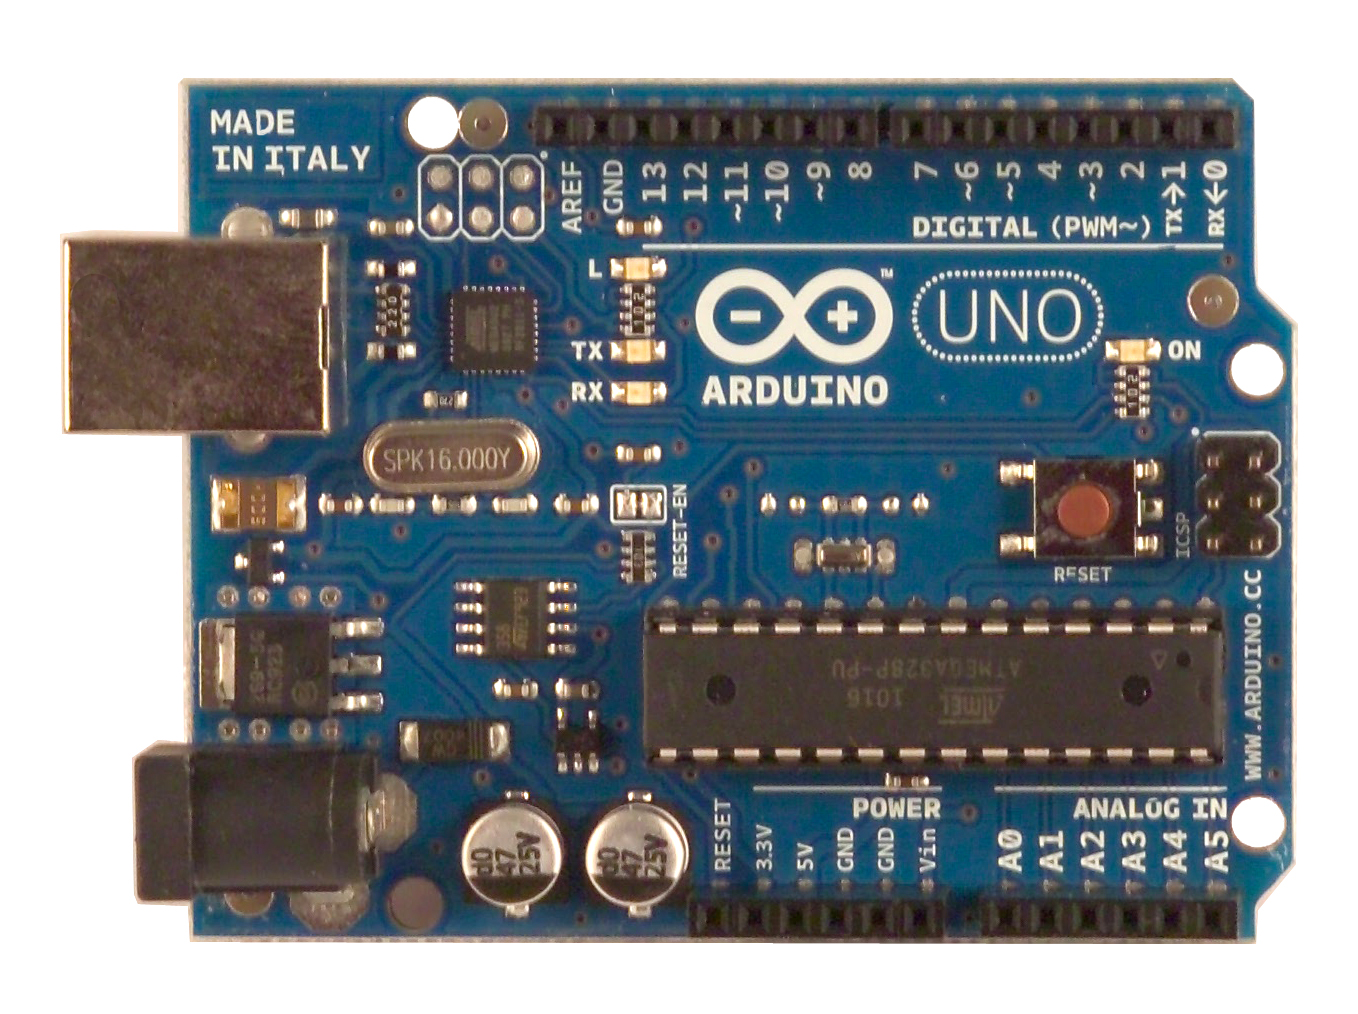
\includegraphics[width=.95\textwidth]{ArduinoUnoFront.jpg}}
      \centerline{Arduino Uno}
    \end{column}
    \begin{column}{0.5\textwidth}
      \pause
      \centerline{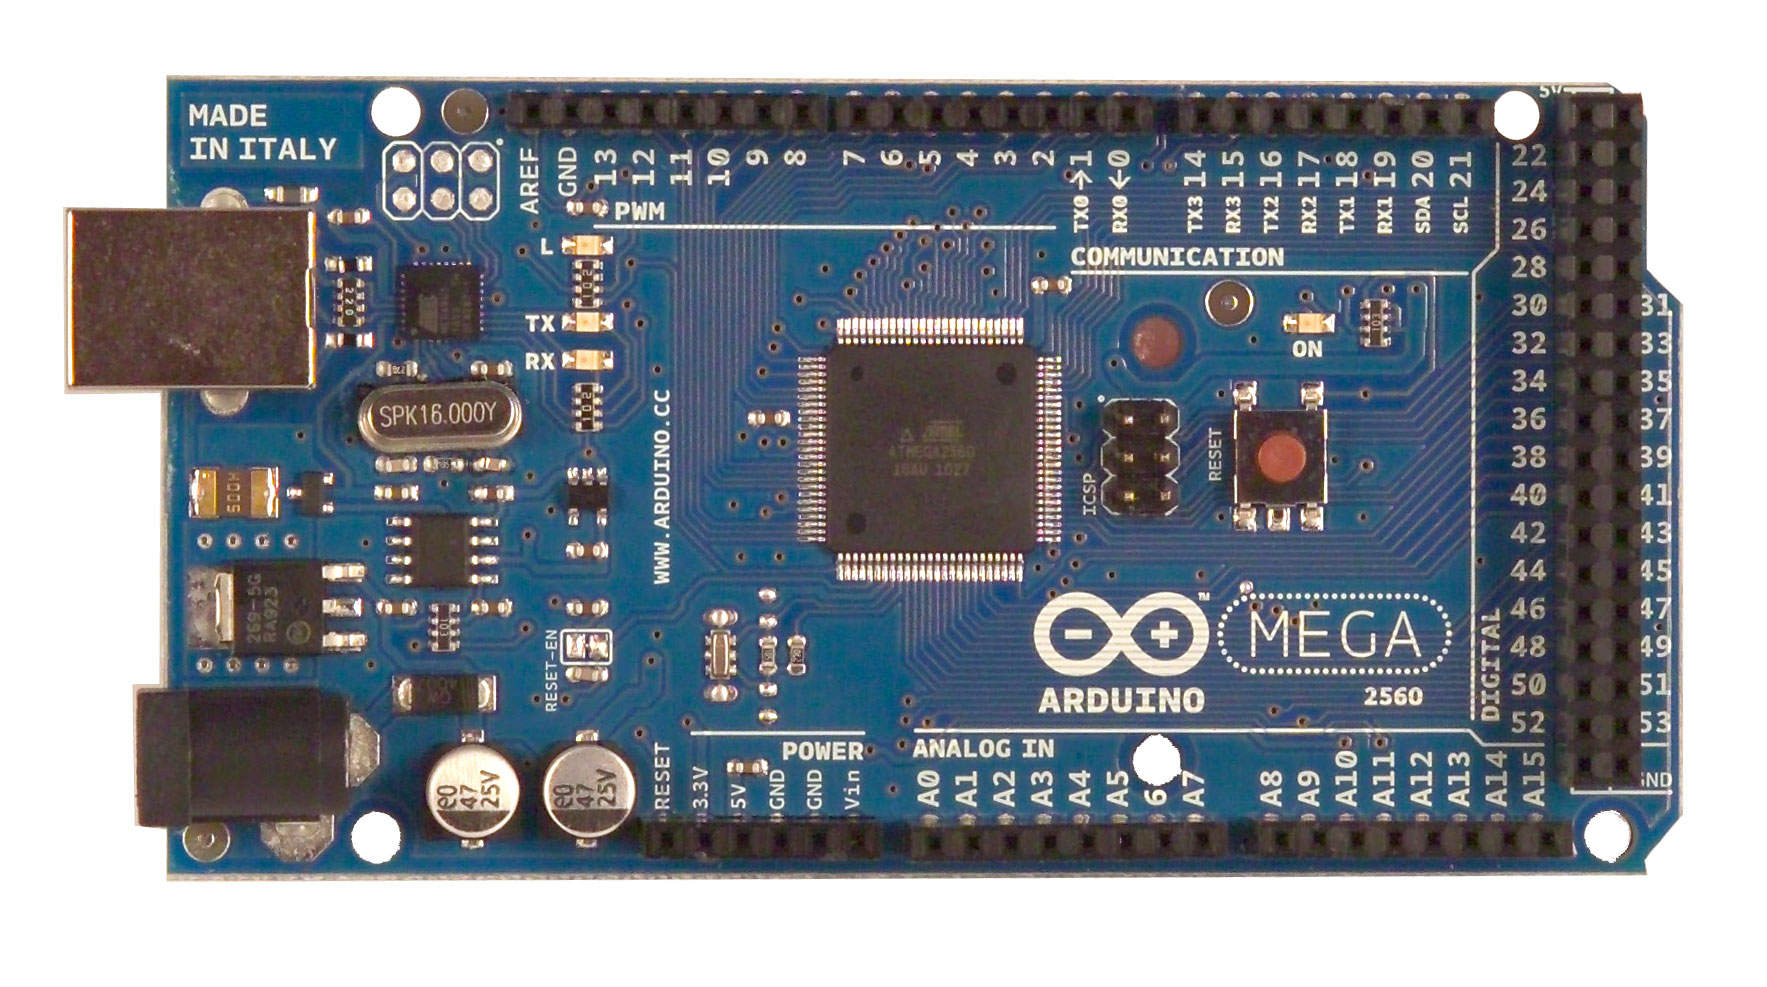
\includegraphics[width=.95\textwidth]{ArduinoMega2650Front.jpg}}
      \centerline{Arduino Mega2560}
    \end{column}
  \end{columns}
\end{frame}

\begin{frame}{Arduino Variations}
  \begin{columns}
    \begin{column}{0.5\textwidth}
      \pause
      \centerline{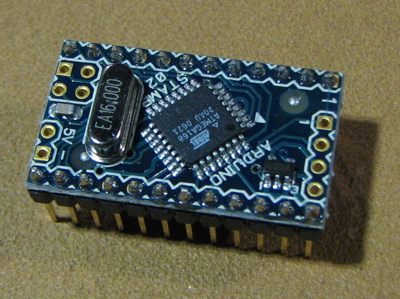
\includegraphics[width=.95\textwidth]{arduino_mini.jpg}}
      \centerline{Arduino Mini}
      \centerline{The smallest Arduino}
    \end{column}
    \begin{column}{0.5\textwidth}
      \pause
      \centerline{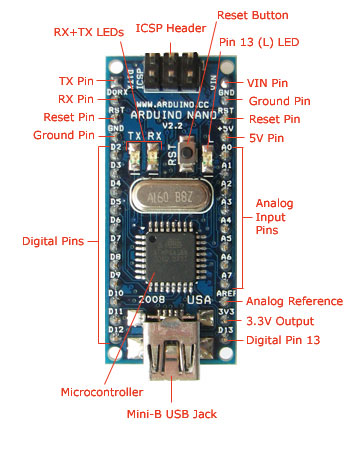
\includegraphics[width=.95\textwidth]{NanoFront.jpg}}
      \centerline{Arduino Nano}
    \end{column}
  \end{columns}
\end{frame}


\begin{frame}{Arduino Variations}
  \begin{columns}
    \begin{column}{0.5\textwidth}
      \pause
      \centerline{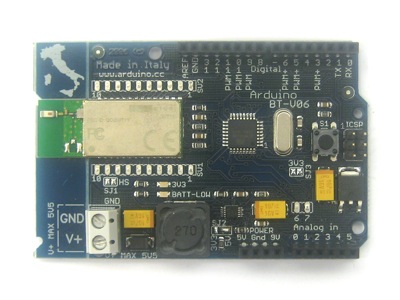
\includegraphics[width=.95\textwidth]{ArduinoBT400.jpg}}
      \centerline{Arduino Bluetooth}
    \end{column}
    \begin{column}{0.5\textwidth}
      \pause
      \centerline{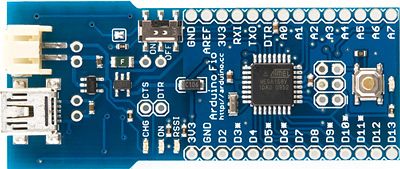
\includegraphics[width=.95\textwidth]{ArduinoFio.jpg}}
      \centerline{Arduino Fio}
    \end{column}
  \end{columns}
\end{frame}

\begin{frame}{Arduino Variations}
  \begin{columns}
    \begin{column}{0.5\textwidth}
      \pause
      \centerline{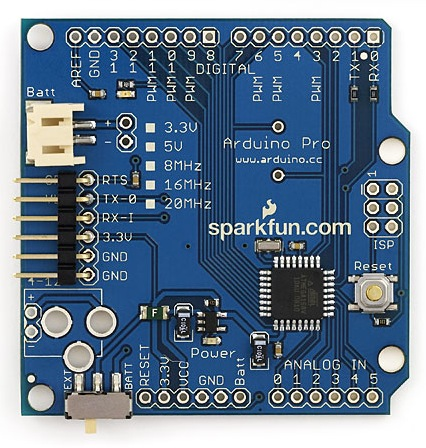
\includegraphics[width=.95\textwidth]{ArduinoPro.jpg}}
      \centerline{Arduino Pro}
    \end{column}
    \begin{column}{0.5\textwidth}
      \pause
      \centerline{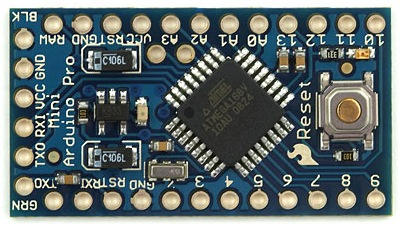
\includegraphics[width=.95\textwidth]{ArduinoProMini.jpg}}
      \centerline{Arduino Pro Mini}
    \end{column}
  \end{columns}
\end{frame}

\begin{frame}{Arduino Variations}
  \centerline{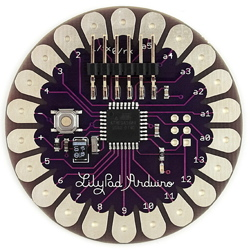
\includegraphics[width=.5\textwidth]{LilyPad_3.jpg}}
  \centerline{Arduino Lilypad}
\end{frame}

\begin{frame}{Arduino Clones}
  \begin{columns}
    \pause
    \begin{column}{0.5\textwidth}
      \centerline{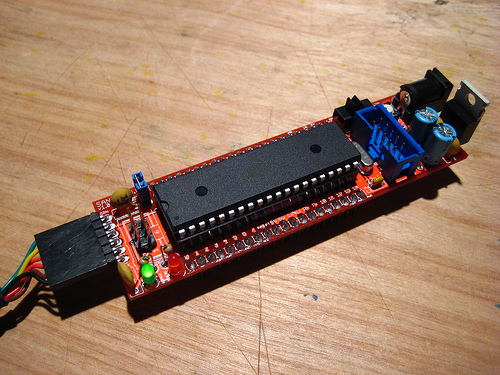
\includegraphics[width=.95\textwidth]{Sanguino.jpg}}
      \centerline{Sanguino}
      \centerline{Uses the ATmega644P}
    \end{column}
    \pause
    \begin{column}{0.5\textwidth}
      \centerline{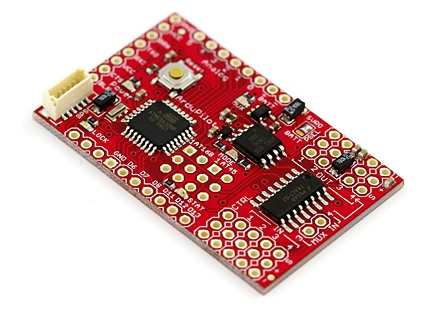
\includegraphics[width=.95\textwidth]{ardupilot.jpg}}
      \centerline{ArduPilot}
    \end{column}
  \end{columns}
\end{frame}

\begin{frame}{Arduino Interaction}
  \centerline{But I want to make my Arduino \emph{do} something.}
  \centerline{How do I get the Arduino to interact with anything?}
  \pause
  \bigskip
  \centerline{The obvious answer:}
  \centerline{Hook some peripheral devices up to the Digital or Analog I/O pins.}
\end{frame}

\begin{frame}{Shields}
  \centerline{The more interesting answer?}
  \pause
  \centerline{Shields}
  \centerline{These are the plugins of the Arduino world}
  \centerline{Allows Arduino users to easily extend their arduino's capabilities}
\end{frame}

\begin{frame}{Shield Examples}
  \begin{columns}
    \pause
    \begin{column}{0.5\textwidth}
      \centerline{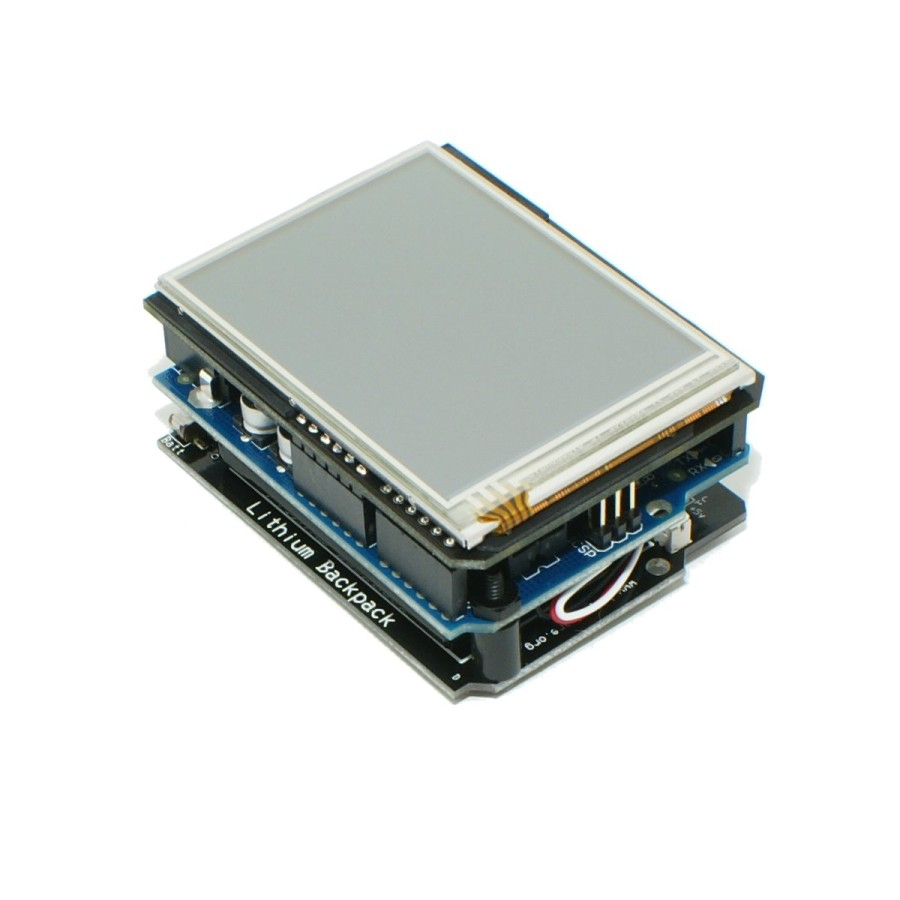
\includegraphics[width=.95\textwidth]{touch_shield.jpg}}
      \centerline{Touch Shield from liquidware}
    \end{column}
    \begin{column}{0.5\textwidth}
      \centerline{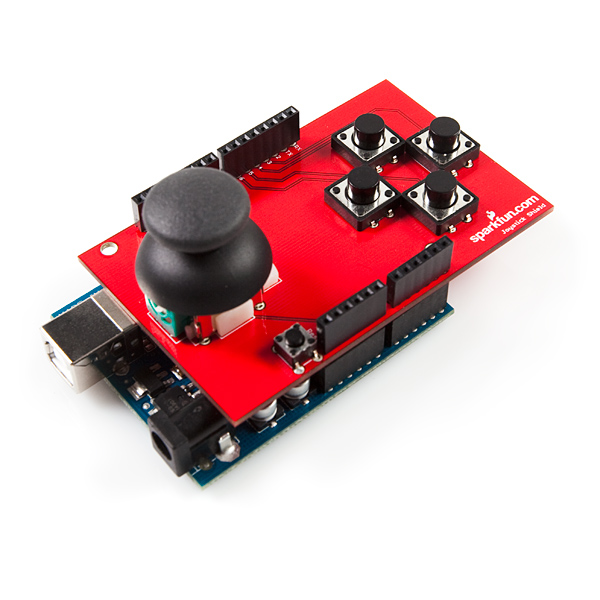
\includegraphics[width=.95\textwidth]{joystick-shield.jpg}}
      \centerline{Joystick Shield}
    \end{column}
  \end{columns}
\end{frame}


\section{Software}
\begin{frame}{Software Overview}
  \centerline{Okay, so there's a lot of hardware}
  \centerline{What about the software side?}
\end{frame}

\begin{frame}{Software Stack}
  \begin{centering}
    \begin{itemize}
      \item Cross Platform IDE
      \item Uses the Wiring library
      \item Uses the GNU toolchain and AVR Libc to compile
      \item Uploads to the Arduino via avrdude
    \end{itemize}
  \end{centering}
\end{frame}

\begin{frame}{Wiring}
  \begin{centering}
    \begin{itemize}
      \item Software library originally written for a project of the same name
      \item C/C++
      \item Provides convenient shortcuts when writing microcontroller code
    \end{itemize}
  \end{centering}
\end{frame}

\begin{frame}{Code}
  \begin{centering}
    Arduino code only two functions to be present in order to run
    \begin{itemize}
      \item void setup() - this gets run at boot time
      \item void loop() - this function is repeatedly called until the board is powered off
    \end{itemize}
  \end{centering}
\end{frame}


\begin{frame}
  \centerline{\huge Questions?}
  \centerline{Comments?}
\end{frame}

\end{document}
